\begin{frame}{Diseño e implementación de modelos.\newline Preparación de los datos I}
	\begin{figure}[ht!]
		\centering
		\resizebox{\textwidth}{!}{
			\begin{tikzpicture}
			\tikzstyle{box} = [draw,inner sep=7,minimum size=57,line 
			width=1, very thick, draw=black, fill=black!20, text width=100, text centered]
			\tikzstyle{invisible} = [outer sep=0,inner sep=0,minimum size=0]
			\tikzstyle{stealth} = [-stealth, very thick]
			\begin{scope}[shift={(0.5,0)}]		
			\begin{scope}[shift={(-3.5,3.1)}, scale=0.5]
			\node [invisible] at (-1.2,1.7) {$FFT_n$};
			\draw (-3,0.5) node [invisible] {} -- (-2.8,0.3) node [invisible] {} -- (-2.6,0.2) node [invisible] {} -- (-2.4,0.8) node [invisible] {} -- (-2.2,0.2) node [invisible] {} -- (-2,0.3) node [invisible] {} -- (-1.9,0.2) node [invisible] {} -- (-1.8,0.4) node [invisible] {} -- (-1.7,0.2) node [invisible] {} -- (-1.6,1.4) node [invisible] {} -- (-1.5,0.2) node [invisible] {} -- (-1.3,0.3) node [invisible] (v4) {};
			\node [invisible] (v2) at (-3,1.6) {};
			\node [invisible] (v1) at (-3,-0.4) {};
			\node [invisible] (v3) at (0.6,-0.4) {};
			\draw [stealth] (v1) edge (v2);
			\draw [stealth] (v1) edge (v3);
			\draw [stealth](v4);
			\draw (v4) -- (-1.2,0.2) node [invisible] {} -- (-1.1,0.4) node [invisible] {} -- (-1,0.2) node [invisible] {} -- (-0.8,0.8) node [invisible] {} -- (-0.7,0.2) node [invisible] {} -- (-0.5,0.3) node [invisible] {} -- (-0.4,0.2) node [invisible] {} -- (-0.2,0.3) node [invisible] {} -- (-0.1,0.2) node [invisible] {} -- (0.1,1.1) node [invisible] {} -- (0.3,0.2) node [invisible] {};
			\end{scope}
			\begin{scope}[shift={(-3.1,1.8)}, scale=0.5]
			\node [invisible] at (-1.2,1.7) {$FFT_{n-1}$};
			\draw (-3,0.5) node [invisible] {} -- (-2.8,0.3) node [invisible] {} -- (-2.6,0.2) node [invisible] {} -- (-2.4,0.8) node [invisible] {} -- (-2.2,0.2) node [invisible] {} -- (-2,0.3) node [invisible] {} -- (-1.9,0.2) node [invisible] {} -- (-1.8,0.4) node [invisible] {} -- (-1.7,0.2) node [invisible] {} -- (-1.6,1.4) node [invisible] {} -- (-1.5,0.2) node [invisible] {} -- (-1.3,0.3) node [invisible] (v4) {};
			\node [invisible] (v2) at (-3,1.6) {};
			\node [invisible] (v1) at (-3,-0.4) {};
			\node [invisible] (v3) at (0.6,-0.4) {};
			\draw [stealth] (v1) edge (v2);
			\draw [stealth] (v1) edge (v3);
			\draw [stealth](v4);
			\draw (v4) -- (-1.2,0.2) node [invisible] {} -- (-1.1,0.4) node [invisible] {} -- (-1,0.2) node [invisible] {} -- (-0.8,0.8) node [invisible] {} -- (-0.7,0.2) node [invisible] {} -- (-0.5,0.3) node [invisible] {} -- (-0.4,0.2) node [invisible] {} -- (-0.2,0.3) node [invisible] {} -- (-0.1,0.2) node [invisible] {} -- (0.1,1.1) node [invisible] {} -- (0.3,0.2) node [invisible] {};
			\end{scope}
			\begin{scope}[shift={(-1.5,-0.9)}, scale=0.5]
			\node [invisible] at (-1.2,1.7) {$FFT_2$};
			\draw (-3,0.5) node [invisible] {} -- (-2.8,0.3) node [invisible] {} -- (-2.6,0.2) node [invisible] {} -- (-2.4,0.8) node [invisible] {} -- (-2.2,0.2) node [invisible] {} -- (-2,0.3) node [invisible] {} -- (-1.9,0.2) node [invisible] {} -- (-1.8,0.4) node [invisible] {} -- (-1.7,0.2) node [invisible] {} -- (-1.6,1.4) node [invisible] {} -- (-1.5,0.2) node [invisible] {} -- (-1.3,0.3) node [invisible] (v4) {};
			\node [invisible] (v2) at (-3,1.6) {};
			\node [invisible] (v1) at (-3,-0.4) {};
			\node [invisible] (v3) at (0.6,-0.4) {};
			\draw [stealth] (v1) edge (v2);
			\draw [stealth] (v1) edge (v3);
			\draw [stealth](v4);
			\draw (v4) -- (-1.2,0.2) node [invisible] {} -- (-1.1,0.4) node [invisible] {} -- (-1,0.2) node [invisible] {} -- (-0.8,0.8) node [invisible] {} -- (-0.7,0.2) node [invisible] {} -- (-0.5,0.3) node [invisible] {} -- (-0.4,0.2) node [invisible] {} -- (-0.2,0.3) node [invisible] {} -- (-0.1,0.2) node [invisible] {} -- (0.1,1.1) node [invisible] {} -- (0.3,0.2) node [invisible] {};
			\end{scope}
			\begin{scope}[shift={(-1.1,-2.2)}, scale=0.5]
			\node [invisible] at (-1.2,1.7) {$FFT_1$};
			\draw (-3,0.5) node [invisible] {} -- (-2.8,0.3) node [invisible] {} -- (-2.6,0.2) node [invisible] {} -- (-2.4,0.8) node [invisible] {} -- (-2.2,0.2) node [invisible] {} -- (-2,0.3) node [invisible] {} -- (-1.9,0.2) node [invisible] {} -- (-1.8,0.4) node [invisible] {} -- (-1.7,0.2) node [invisible] {} -- (-1.6,1.4) node [invisible] {} -- (-1.5,0.2) node [invisible] {} -- (-1.3,0.3) node [invisible] (v4) {};
			\node [invisible] (v2) at (-3,1.6) {};
			\node [invisible] (v1) at (-3,-0.4) {};
			\node [invisible] (v3) at (0.6,-0.4) {};
			\draw [stealth] (v1) edge (v2);
			\draw [stealth] (v1) edge (v3);
			\draw [stealth](v4);
			\draw (v4) -- (-1.2,0.2) node [invisible] {} -- (-1.1,0.4) node [invisible] {} -- (-1,0.2) node [invisible] {} -- (-0.8,0.8) node [invisible] {} -- (-0.7,0.2) node [invisible] {} -- (-0.5,0.3) node [invisible] {} -- (-0.4,0.2) node [invisible] {} -- (-0.2,0.3) node [invisible] {} -- (-0.1,0.2) node [invisible] {} -- (0.1,1.1) node [invisible] {} -- (0.3,0.2) node [invisible] {};
			\end{scope}
			\node [circle, fill] at (-3.6,1.2) {};
			\node [circle, fill] at (-3.2,0.8) {};
			\node [circle, fill] at (-2.8,0.4) {};
			\draw [dashed, thick] (-5.5,6) node [invisible] (v5) {} -- (-5.5,-3.5) -- (-0.5,-3.5) -- (-0.5,6) -- (v5);
			\node [invisible] (v6) at (-0.5,0.75) {};
			\end{scope}
			
			\begin{scope}[shift={(10.5,0)}]		
			\begin{scope}[shift={(-1.2,3.1)}, scale=0.5]
			\node [invisible] at (-1.2,1.7) {$FFT_n$};
			\draw (-3,0.5) node [invisible] {} -- (-2.8,0.3) node [invisible] {} -- (-2.6,0.2) node [invisible] {} -- (-2.4,0.8) node [invisible] {} -- (-2.2,0.2) node [invisible] {} -- (-2,0.3) node [invisible] {} -- (-1.9,0.2) node [invisible] {} -- (-1.8,0.4) node [invisible] {} -- (-1.7,0.2) node [invisible] {} -- (-1.6,1.4) node [invisible] {} -- (-1.5,0.2) node [invisible] {} -- (-1.3,0.3) node [invisible] (v4) {};
			\node [invisible] (v2) at (-3,1.6) {};
			\node [invisible] (v1) at (-3,-0.4) {};
			\node [invisible] (v3) at (0.6,-0.4) {};
			\draw [stealth] (v1) edge (v2);
			\draw [stealth] (v1) edge (v3);
			\draw [stealth](v4);
			\draw (v4) -- (-1.2,0.2) node [invisible] {} -- (-1.1,0.4) node [invisible] {} -- (-1,0.2) node [invisible] {} -- (-0.8,0.8) node [invisible] {} -- (-0.7,0.2) node [invisible] {} -- (-0.5,0.3) node [invisible] {} -- (-0.4,0.2) node [invisible] {} -- (-0.2,0.3) node [invisible] {} -- (-0.1,0.2) node [invisible] {} -- (0.1,1.1) node [invisible] {} -- (0.3,0.2) node [invisible] {};
			\end{scope}
			\begin{scope}[shift={(-1.7,1.8)}, scale=0.5]
			\node [invisible] at (-1.2,1.7) {$FFT_{n-1}$};
			\draw (-3,0.5) node [invisible] {} -- (-2.8,0.3) node [invisible] {} -- (-2.6,0.2) node [invisible] {} -- (-2.4,0.8) node [invisible] {} -- (-2.2,0.2) node [invisible] {} -- (-2,0.3) node [invisible] {} -- (-1.9,0.2) node [invisible] {} -- (-1.8,0.4) node [invisible] {} -- (-1.7,0.2) node [invisible] {} -- (-1.6,1.4) node [invisible] {} -- (-1.5,0.2) node [invisible] {} -- (-1.3,0.3) node [invisible] (v4) {};
			\node [invisible] (v2) at (-3,1.6) {};
			\node [invisible] (v1) at (-3,-0.4) {};
			\node [invisible] (v3) at (0.6,-0.4) {};
			\draw [stealth] (v1) edge (v2);
			\draw [stealth] (v1) edge (v3);
			\draw [stealth](v4);
			\draw (v4) -- (-1.2,0.2) node [invisible] {} -- (-1.1,0.4) node [invisible] {} -- (-1,0.2) node [invisible] {} -- (-0.8,0.8) node [invisible] {} -- (-0.7,0.2) node [invisible] {} -- (-0.5,0.3) node [invisible] {} -- (-0.4,0.2) node [invisible] {} -- (-0.2,0.3) node [invisible] {} -- (-0.1,0.2) node [invisible] {} -- (0.1,1.1) node [invisible] {} -- (0.3,0.2) node [invisible] {};
			\end{scope}
			\begin{scope}[shift={(-3.2,-0.9)}, scale=0.5]
			\node [invisible] at (-1.2,1.7) {$FFT_2$};
			\draw (-3,0.5) node [invisible] {} -- (-2.8,0.3) node [invisible] {} -- (-2.6,0.2) node [invisible] {} -- (-2.4,0.8) node [invisible] {} -- (-2.2,0.2) node [invisible] {} -- (-2,0.3) node [invisible] {} -- (-1.9,0.2) node [invisible] {} -- (-1.8,0.4) node [invisible] {} -- (-1.7,0.2) node [invisible] {} -- (-1.6,1.4) node [invisible] {} -- (-1.5,0.2) node [invisible] {} -- (-1.3,0.3) node [invisible] (v4) {};
			\node [invisible] (v2) at (-3,1.6) {};
			\node [invisible] (v1) at (-3,-0.4) {};
			\node [invisible] (v3) at (0.6,-0.4) {};
			\draw [stealth] (v1) edge (v2);
			\draw [stealth] (v1) edge (v3);
			\draw [stealth](v4);
			\draw (v4) -- (-1.2,0.2) node [invisible] {} -- (-1.1,0.4) node [invisible] {} -- (-1,0.2) node [invisible] {} -- (-0.8,0.8) node [invisible] {} -- (-0.7,0.2) node [invisible] {} -- (-0.5,0.3) node [invisible] {} -- (-0.4,0.2) node [invisible] {} -- (-0.2,0.3) node [invisible] {} -- (-0.1,0.2) node [invisible] {} -- (0.1,1.1) node [invisible] {} -- (0.3,0.2) node [invisible] {};
			\end{scope}
			\begin{scope}[shift={(-3.7,-2.2)}, scale=0.5]
			\node [invisible] at (-1.2,1.7) {$FFT_1$};
			\draw (-3,0.5) node [invisible] {} -- (-2.8,0.3) node [invisible] {} -- (-2.6,0.2) node [invisible] {} -- (-2.4,0.8) node [invisible] {} -- (-2.2,0.2) node [invisible] {} -- (-2,0.3) node [invisible] {} -- (-1.9,0.2) node [invisible] {} -- (-1.8,0.4) node [invisible] {} -- (-1.7,0.2) node [invisible] {} -- (-1.6,1.4) node [invisible] {} -- (-1.5,0.2) node [invisible] {} -- (-1.3,0.3) node [invisible] (v4) {};
			\node [invisible] (v2) at (-3,1.6) {};
			\node [invisible] (v1) at (-3,-0.4) {};
			\node [invisible] (v3) at (0.6,-0.4) {};
			\draw [stealth] (v1) edge (v2);
			\draw [stealth] (v1) edge (v3);
			\draw [stealth](v4);
			\draw (v4) -- (-1.2,0.2) node [invisible] {} -- (-1.1,0.4) node [invisible] {} -- (-1,0.2) node [invisible] {} -- (-0.8,0.8) node [invisible] {} -- (-0.7,0.2) node [invisible] {} -- (-0.5,0.3) node [invisible] {} -- (-0.4,0.2) node [invisible] {} -- (-0.2,0.3) node [invisible] {} -- (-0.1,0.2) node [invisible] {} -- (0.1,1.1) node [invisible] {} -- (0.3,0.2) node [invisible] {};
			\end{scope}
			\node [circle, fill] at (-2.8,1.2) {};
			\node [circle, fill] at (-3.2,0.8) {};
			\node [circle, fill] at (-3.6,0.4) {};
			\draw [dashed, thick] (-5.5,6) node [invisible] (v5) {} -- (-5.5,-3.5) -- (-0.5,-3.5) -- (-0.5,6) -- (v5);
			\node [invisible] (v8) at (-5.5,0.75) {};
			\end{scope}
			
			\node [box,text width=60] (v7) at (2.5,0.75) {Modelo};
			
			
			\node [invisible] at (-2.5,5.5) {Módulo de FFT con ruido};
			\node [invisible] at (7.5,5.5) {Módulo de FFT sin ruido};
			\draw [stealth] (v6) edge (v7);
			\draw [stealth] (v7) edge (v8);
			\node [box] (v9) at (-8.5,7) {$Tiempo\xrightarrow{FFT}Frecuencia$};
			\node [box] (v10) at (13.5,7) {$Frecuencia\xrightarrow{iFFT}Tiempo$};
			\node [invisible] (v11) at (-5,0.75) {};
			\node [invisible] (v12) at (10,0.75) {};
			\draw [stealth,out=0,in=180] (v9) edge node[anchor=south]{Fase} (v10);
			\draw [stealth,out=0,in=180] (v9) edge node[anchor=east]{Módulo}(v11);
			\draw [stealth,out=0,in=180] (v12) edge node[anchor=west]{Módulo}(v10);
			\end{tikzpicture}
		}      
		\caption{Esquema de las entradas y salidas de datos del modelo}
		\label{fig: model_schema}
	\end{figure}
\end{frame}
\begin{frame}{Diseño e implementación de modelos.\newline Preparación de los datos II}
	\begin{figure}[ht!]
		\centering
		\resizebox{\textwidth}{!}{
			\begin{tikzpicture}
			\tikzstyle{box} = [draw,inner sep=7,minimum size=57,line 
			width=1, very thick, draw=black, fill=black!20, text width=80, text centered]
			\tikzstyle{invisible} = [outer sep=0,inner sep=0,minimum size=0]
			\tikzstyle{stealth} = [-stealth, very thick]
			\begin{scope} [scale=0.1, shift={(-112.5,10)}]
			\draw [very thick] (-2,0.5) arc (0:-180:1.5);
			\draw [very thick] (-2,3.5) arc (0:180:1.5);
			\node [invisible] (v1) at (-5,3.5) {};
			\node [invisible] (v3) at (-2,3.5) {};
			\node [invisible] (v2) at (-5,0.5) {};
			\node [invisible] (v4) at (-2,0.5) {};
			\draw [very thick] (v1) edge (v2);
			\draw [very thick] (v3) edge (v4);
			\node [invisible] (v9) at (-5,3) {};
			\node [invisible] (v10) at (-4,3) {};
			\node [invisible] (v11) at (-5,2) {};
			\node [invisible] (v12) at (-4,2) {};
			\node [invisible] (v13) at (-5,1) {};
			\node [invisible] (v14) at (-4,1) {};
			\node [invisible] (v15) at (-2,1) {};
			\node [invisible] (v16) at (-3,1) {};
			\node [invisible] (v17) at (-2,2) {};
			\node [invisible] (v18) at (-3,2) {};
			\node [invisible] (v19) at (-2,3) {};
			\node [invisible] (v20) at (-3,3) {};
			\draw [very thick] (-1.5,0.5) arc (0:-180:2);
			\node [invisible] (v7) at (-3.5,-1.5) {};
			\node [invisible] (v8) at (-3.5,-2.5) {};
			\node [invisible] (v5) at (-5.5,-2.5) {};
			\node [invisible] (v6) at (-1.5,-2.5) {};
			\draw [very thick] (v5) edge (v6);
			\draw [very thick] (v7) edge (v8);
			\draw [very thick] (v9) edge (v10);
			\draw [very thick] (v11) edge (v12);
			\draw [very thick] (v13) edge (v14);
			\draw [very thick] (v15) edge (v16);
			\draw [very thick] (v17) edge (v18);
			\draw [very thick] (v19) edge (v20);
			\end{scope}
			\node [box] (v23) at (-3,1) {Adaptación de la tasa de muestreo a $11025 \frac{muestras}{segundo}$};
			\node [box] (v22) at (-8.1,1) {Analógico $\xrightarrow{}$ Digital};
			\node [invisible] (v21) at (-11,1) {};
			\node [box] (v24) at (2.5,1) {FFT de $1024~muestras$};
			\node [box, minimum size=40] (v30) at (8.5,2.5) {Módulo};
			\node [box, minimum size=40] (v31) at (8.5,-0.5) {Fase};
			\node [box] (v26) at (2.5,-4.5) {$mod\cdot e^{j\cdot fase}$};
			\node [box] (v27) at (-3,-4.5) {iFFT};
			\node [box] (v28) at (-8.1,-4.5) {Analógico $\xleftarrow{}$ Digital};
			\begin{scope}[scale=0.4, shift={(-35.6,-8.15)}, xscale=-1]
			\draw [rounded corners, very thick, fill] (-7,-2.6) node [invisible] (v25) {} -- (-7,-3.6) node [invisible] {} -- (-6.5,-3.5) node [invisible] {} -- (-5.5,-4.5) node [invisible] {} -- (-5.5,-1.5) node [invisible] {} -- (-6.5,-2.5) node [invisible] {} -- (v25);
			\draw [very thick] (-5.0603,-2.658) arc (19.9988:-20:1);
			\draw [very thick] (-4.5905,-2.487) arc (19.9994:-20:1.5);
			\draw [very thick] (-4.1206,-2.316) arc (19.9988:-20:2);
			\draw [very thick] (-3.6508,-2.1449) arc (20.0013:-20:2.5);
			\end{scope}
			\node [invisible] (v29) at (-11,-4.5) {};
			\node [box, minimum size=40] (v32) at (8.5,-5) {Red neuronal recurrente};
			\draw [stealth] (v21) edge node [anchor=south]{$x_{in}(t)$} (v22);
			\draw [stealth] (v22) edge node [anchor=south]{$x_{in}(n)$}(v23);
			\draw [stealth] (v23) edge node [anchor=south]{$\widetilde{x_{in}}(n)$} (v24);
			\draw [stealth,out=0,in=180] (v24) edge node [anchor=north west]{$FFT(n)$} (v30);
			\draw [stealth, out=0, in=180] (v24) edge (v31);
			\draw [stealth,out=0,in=0] (v30) edge node [anchor=east]{$mod(n)$} (v32);
			\draw [stealth] (v32) edge node [anchor=north]{$\widetilde{mod}(n)$} (v26);
			\draw [stealth] (v26) edge node [anchor=south]{$imag_(n)$} (v27);
			\draw [stealth] (v27) edge node [anchor=south]{$x_{out}(n)$} (v28);
			\draw [stealth] (v28) edge node [anchor=south]{$x_{out}(t)$} (v29);
			\node [invisible] (v33) at (10.5,-3) {};
			\draw [very thick, out=0, in=15] (v31) edge (v33);
			\draw [stealth] (v33) edge node [anchor=south]{$fase(n)$} (v26);
			\end{tikzpicture}
		}      
		\caption{Cadena completa de procesado de señal}
		\label{fig: model_chain}
	\end{figure}
	\vspace*{-15pt}
	\begin{itemize}
		\item Cálculo de las FFTs:
		\begin{itemize}
			\scriptsize
			\item Tasa de muestreo: 11025 sps
			\item Tamaño FFT: 1024 muestras (513 bandas de 10.74Hz)
			\item Overlap: 50\%
			
				\vspace*{5pt}
				\resizebox{0.2\textwidth}{!}{
					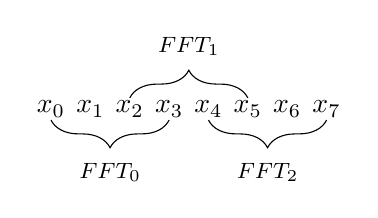
\begin{tikzpicture}
					\tikzstyle{box} = [draw,inner sep=7,minimum size=57,line 
					width=1, very thick, draw=black, fill=black!20, text width=100, text centered]
					\tikzstyle{invisible} = [outer sep=0,inner sep=0,minimum size=0]
					\tikzstyle{stealth} = [-stealth, very thick]
					
					\node [] at (-4,0) {$x_0$};
					\node [] at (-3.5,0) {$x_1$};
					\node [] at (-3,0) {$x_2$};
					\node [] at (-2.5,0) {$x_3$};
					\node [] at (-2,0) {$x_4$};
					\node [] at (-1.5,0) {$x_5$};
					\node [] at (-1,0) {$x_6$};
					\node [] at (-0.5,0) {$x_7$};
					
					\draw [decorate,decoration={brace,amplitude=10pt,mirror,raise=4pt},yshift=0pt] (-4,0) -- (-2.5,0) node [black,midway,yshift=-0.8cm] {\footnotesize $FFT_0$};
					\draw [decorate,decoration={brace,amplitude=10pt,mirror,raise=4pt},yshift=0pt] (-1.5,0) -- (-3,0) node [black,midway,yshift=0.8cm] {\footnotesize $FFT_1$};
					\draw [decorate,decoration={brace,amplitude=10pt,mirror,raise=4pt},yshift=0pt] (-2,0) -- (-0.5,0) node [black,midway,yshift=-0.8cm] {\footnotesize $FFT_2$};
					\end{tikzpicture}
				}
			\item Enventanado Hann
		\end{itemize}
		\item Almacenado en HDF5 
	\end{itemize}
\end{frame}
\begin{frame}{Diseño e implementación de modelos.\newline Preparación de los datos III}
	\begin{figure}[h!]
		\centering
		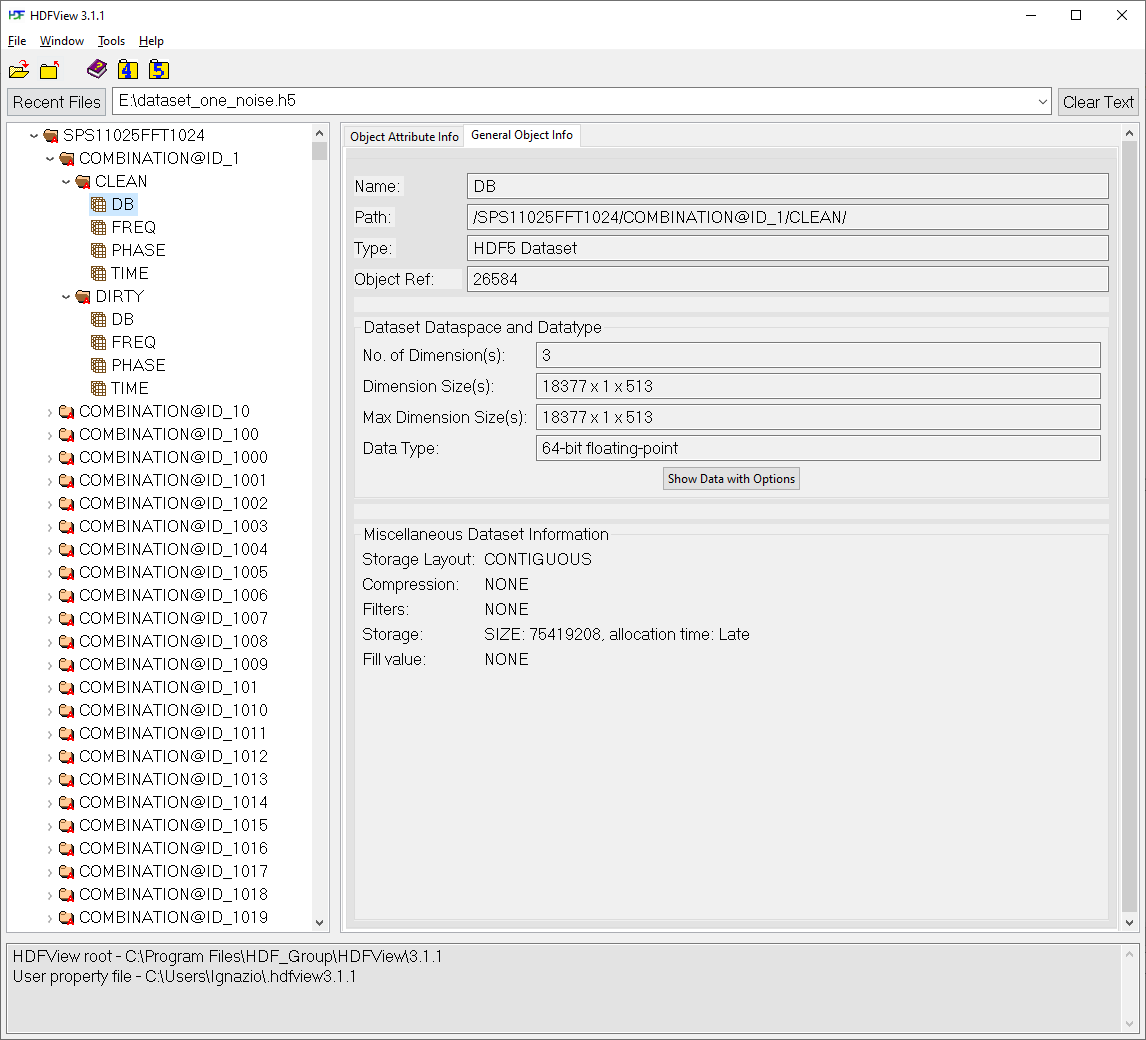
\includegraphics[width=0.75\columnwidth]{../figures/HDF5_struct2}
		\caption{Estructura de los datos almacenados en el archivo HDF5}
		\label{fig: hdf5_struct2}
	\end{figure}
\end{frame}